% Options for packages loaded elsewhere
\PassOptionsToPackage{unicode}{hyperref}
\PassOptionsToPackage{hyphens}{url}
\PassOptionsToPackage{dvipsnames,svgnames,x11names}{xcolor}
\documentclass[
  english,
  man, noextraspace,floatsintext]{apa6}
\usepackage{xcolor}
\usepackage{amsmath,amssymb}
\setcounter{secnumdepth}{-\maxdimen} % remove section numbering
\usepackage{iftex}
\ifPDFTeX
  \usepackage[T1]{fontenc}
  \usepackage[utf8]{inputenc}
  \usepackage{textcomp} % provide euro and other symbols
\else % if luatex or xetex
  \usepackage{unicode-math} % this also loads fontspec
  \defaultfontfeatures{Scale=MatchLowercase}
  \defaultfontfeatures[\rmfamily]{Ligatures=TeX,Scale=1}
\fi
\usepackage{lmodern}
\ifPDFTeX\else
  % xetex/luatex font selection
\fi
% Use upquote if available, for straight quotes in verbatim environments
\IfFileExists{upquote.sty}{\usepackage{upquote}}{}
\IfFileExists{microtype.sty}{% use microtype if available
  \usepackage[]{microtype}
  \UseMicrotypeSet[protrusion]{basicmath} % disable protrusion for tt fonts
}{}
\makeatletter
\@ifundefined{KOMAClassName}{% if non-KOMA class
  \IfFileExists{parskip.sty}{%
    \usepackage{parskip}
  }{% else
    \setlength{\parindent}{0pt}
    \setlength{\parskip}{6pt plus 2pt minus 1pt}}
}{% if KOMA class
  \KOMAoptions{parskip=half}}
\makeatother
% Make \paragraph and \subparagraph free-standing
\makeatletter
\ifx\paragraph\undefined\else
  \let\oldparagraph\paragraph
  \renewcommand{\paragraph}{
    \@ifstar
      \xxxParagraphStar
      \xxxParagraphNoStar
  }
  \newcommand{\xxxParagraphStar}[1]{\oldparagraph*{#1}\mbox{}}
  \newcommand{\xxxParagraphNoStar}[1]{\oldparagraph{#1}\mbox{}}
\fi
\ifx\subparagraph\undefined\else
  \let\oldsubparagraph\subparagraph
  \renewcommand{\subparagraph}{
    \@ifstar
      \xxxSubParagraphStar
      \xxxSubParagraphNoStar
  }
  \newcommand{\xxxSubParagraphStar}[1]{\oldsubparagraph*{#1}\mbox{}}
  \newcommand{\xxxSubParagraphNoStar}[1]{\oldsubparagraph{#1}\mbox{}}
\fi
\makeatother
\usepackage{graphicx}
\makeatletter
\newsavebox\pandoc@box
\newcommand*\pandocbounded[1]{% scales image to fit in text height/width
  \sbox\pandoc@box{#1}%
  \Gscale@div\@tempa{\textheight}{\dimexpr\ht\pandoc@box+\dp\pandoc@box\relax}%
  \Gscale@div\@tempb{\linewidth}{\wd\pandoc@box}%
  \ifdim\@tempb\p@<\@tempa\p@\let\@tempa\@tempb\fi% select the smaller of both
  \ifdim\@tempa\p@<\p@\scalebox{\@tempa}{\usebox\pandoc@box}%
  \else\usebox{\pandoc@box}%
  \fi%
}
% Set default figure placement to htbp
\def\fps@figure{htbp}
\makeatother
% definitions for citeproc citations
\NewDocumentCommand\citeproctext{}{}
\NewDocumentCommand\citeproc{mm}{%
  \begingroup\def\citeproctext{#2}\cite{#1}\endgroup}
\makeatletter
 % allow citations to break across lines
 \let\@cite@ofmt\@firstofone
 % avoid brackets around text for \cite:
 \def\@biblabel#1{}
 \def\@cite#1#2{{#1\if@tempswa , #2\fi}}
\makeatother
\newlength{\cslhangindent}
\setlength{\cslhangindent}{1.5em}
\newlength{\csllabelwidth}
\setlength{\csllabelwidth}{3em}
\newenvironment{CSLReferences}[2] % #1 hanging-indent, #2 entry-spacing
 {\begin{list}{}{%
  \setlength{\itemindent}{0pt}
  \setlength{\leftmargin}{0pt}
  \setlength{\parsep}{0pt}
  % turn on hanging indent if param 1 is 1
  \ifodd #1
   \setlength{\leftmargin}{\cslhangindent}
   \setlength{\itemindent}{-1\cslhangindent}
  \fi
  % set entry spacing
  \setlength{\itemsep}{#2\baselineskip}}}
 {\end{list}}
\usepackage{calc}
\newcommand{\CSLBlock}[1]{\hfill\break\parbox[t]{\linewidth}{\strut\ignorespaces#1\strut}}
\newcommand{\CSLLeftMargin}[1]{\parbox[t]{\csllabelwidth}{\strut#1\strut}}
\newcommand{\CSLRightInline}[1]{\parbox[t]{\linewidth - \csllabelwidth}{\strut#1\strut}}
\newcommand{\CSLIndent}[1]{\hspace{\cslhangindent}#1}
\ifLuaTeX
\usepackage[bidi=basic,shorthands=off]{babel}
\else
\usepackage[bidi=default,shorthands=off]{babel}
\fi
\ifLuaTeX
  \usepackage{selnolig} % disable illegal ligatures
\fi
\setlength{\emergencystretch}{3em} % prevent overfull lines
\providecommand{\tightlist}{%
  \setlength{\itemsep}{0pt}\setlength{\parskip}{0pt}}
% Manuscript styling
\usepackage{upgreek}
\captionsetup{font=singlespacing,justification=justified}

% Table formatting
\usepackage{longtable}
\usepackage{lscape}
% \usepackage[counterclockwise]{rotating}   % Landscape page setup for large tables
\usepackage{multirow}		% Table styling
\usepackage{tabularx}		% Control Column width
\usepackage[flushleft]{threeparttable}	% Allows for three part tables with a specified notes section
\usepackage{threeparttablex}            % Lets threeparttable work with longtable

% Create new environments so endfloat can handle them
% \newenvironment{ltable}
%   {\begin{landscape}\centering\begin{threeparttable}}
%   {\end{threeparttable}\end{landscape}}
\newenvironment{lltable}{\begin{landscape}\centering\begin{ThreePartTable}}{\end{ThreePartTable}\end{landscape}}

% Enables adjusting longtable caption width to table width
% Solution found at http://golatex.de/longtable-mit-caption-so-breit-wie-die-tabelle-t15767.html
\makeatletter
\newcommand\LastLTentrywidth{1em}
\newlength\longtablewidth
\setlength{\longtablewidth}{1in}
\newcommand{\getlongtablewidth}{\begingroup \ifcsname LT@\roman{LT@tables}\endcsname \global\longtablewidth=0pt \renewcommand{\LT@entry}[2]{\global\advance\longtablewidth by ##2\relax\gdef\LastLTentrywidth{##2}}\@nameuse{LT@\roman{LT@tables}} \fi \endgroup}

% \setlength{\parindent}{0.5in}
% \setlength{\parskip}{0pt plus 0pt minus 0pt}

% Overwrite redefinition of paragraph and subparagraph by the default LaTeX template
% See https://github.com/crsh/papaja/issues/292
\makeatletter
\renewcommand{\paragraph}{\@startsection{paragraph}{4}{\parindent}%
  {0\baselineskip \@plus 0.2ex \@minus 0.2ex}%
  {-1em}%
  {\normalfont\normalsize\bfseries\itshape\typesectitle}}

\renewcommand{\subparagraph}[1]{\@startsection{subparagraph}{5}{1em}%
  {0\baselineskip \@plus 0.2ex \@minus 0.2ex}%
  {-\z@\relax}%
  {\normalfont\normalsize\itshape\hspace{\parindent}{#1}\textit{\addperi}}{\relax}}
\makeatother

\makeatletter
\usepackage{etoolbox}
\patchcmd{\maketitle}
  {\section{\normalfont\normalsize\abstractname}}
  {\section*{\normalfont\normalsize\abstractname}}
  {}{\typeout{Failed to patch abstract.}}
\patchcmd{\maketitle}
  {\section{\protect\normalfont{\@title}}}
  {\section*{\protect\normalfont{\@title}}}
  {}{\typeout{Failed to patch title.}}
\makeatother

\usepackage{xpatch}
\makeatletter
\xapptocmd\appendix
  {\xapptocmd\section
    {\addcontentsline{toc}{section}{\appendixname\ifoneappendix\else~\theappendix\fi: #1}}
    {}{\InnerPatchFailed}%
  }
{}{\PatchFailed}
\makeatother
\keywords{meta-analysis, mixture model, latent class analysis, random effects\newline\indent Word count: 5423}
\usepackage{lineno}

\linenumbers
\usepackage{csquotes}
\usepackage{longtable, setspace, subfig}
\raggedbottom
\usepackage{bookmark}
\IfFileExists{xurl.sty}{\usepackage{xurl}}{} % add URL line breaks if available
\urlstyle{same}
\hypersetup{
  pdftitle={When One Random Effect Is Not Enough: Mixture Model Meta-Analysis},
  pdfauthor={Caspar J. Van Lissa1},
  pdflang={en-EN},
  pdfkeywords={meta-analysis, mixture model, latent class analysis, random effects},
  colorlinks=true,
  linkcolor={Maroon},
  filecolor={Maroon},
  citecolor={Blue},
  urlcolor={blue},
  pdfcreator={LaTeX via pandoc}}

\title{When One Random Effect Is Not Enough: Mixture Model Meta-Analysis}
\author{Caspar J. Van Lissa\textsuperscript{1}}
\date{}


\shorttitle{MIXTURE META-ANALYSIS}

\authornote{

This is a preprint paper, generated from Git Commit \# d03ab61a.

The authors made the following contributions. Caspar J. Van Lissa: Conceptualization, Formal Analysis, Funding acquisition, Methodology, Project administration, Software, Supervision, Writing -- original draft, Writing -- review \& editing.

Correspondence concerning this article should be addressed to Caspar J. Van Lissa, Professor Cobbenhagenlaan 125, 5037 DB Tilburg, The Netherlands. E-mail: \href{mailto:c.j.vanlissa@tilburguniversity.edu}{\nolinkurl{c.j.vanlissa@tilburguniversity.edu}}

}

\affiliation{\vspace{0.5cm}\textsuperscript{1} Tilburg University, dept. Methodology \& Statistics}

\abstract{%
Handling between-study differences in effect sizes, or heterogeneity, is a key challenge in meta-analysis.
The common assumption that heterogeneity is normally distributed implies an absence of systematic sources of heterogeneity, or known and measured sources of heterogeneity that can be controlled using moderator analysis.
These assumptions fall short when effect sizes originate from multiple unknown subpopulations - for example, due to different research traditions, unmeasured moderators, publication bias, and outliers.
It has been argued that finite mixture models - also known as latent class analysis (LCA) - can capture these unobserved subgroups,
but there is currently no generalized framework for estimating such models.
We introduce open source software for estimating random-effects mixture, or ``remix'' meta-analyses.
Implemented in \texttt{OpenMx}, these structural equation models can be fully customized and further extended.
We conducted a simulation study to evaluate the \texttt{remix} algorithm's convergence, bias and confidence interval coverage,
and the performance of four class enumeration metrics (the AIC, BIC, and ICL information criteria, and predictive model comparison or PMC).
Results show that the method is fast and has low bias, but confidence interval coverage is below nominal levels,
and class enumeration remains challenging - which are known limitations of LCA.
Nevertheless, remix meta-analysis is the appropriate method when effect sizes originate from a mixture of unobserved subpopulations; a scenario which is arguably commonplace in meta-analysis.
}



\begin{document}
\maketitle

When synthesizing effect sizes originating from different studies, a key question is how to properly account for between-study differences.
The choice of an appropriate statistical model depends on theoretical assumptions about the sources of heterogeneity.
For example, the \emph{fixed-effect} model assumes no differences in true effect size.
If our effect sizes result from close replications of a particular experiment, it is sensible to assume one true population effect, which implies that any differences between observed effect sizes must be due to sampling error.
If our effect sizes instead result from a wide range of different studies, conducted in different labs with unique designs and distinct measures - then we might expert there to be variance in true effect sizes.
If we assume that there are no systematic differences, then the \emph{random effects} model can estimate the variance of true effect sizes, \(\tau^2\).
If we know that there are systematic sources of heterogeneity, for example, because some studies used a stronger manipulation than others, and we have coded these sources as moderator variables, then we can control for these differences using \emph{meta-regression}.
And finally, if we suspect that there are systematic sources of heterogeneity, but we don't know which moderator variables are relevant, machine learning methods meta-regression can be used to perform variable selection, retaining only the relevant moderators (Caspar J. Van Lissa, 2020; Caspar J. Van Lissa, van Erp, \& Clapper, 2023).
Thus, there are well-established methods for situations where there is no heterogeneity, random heterogeneity, or heterogeneity due to known and measured moderators.

A scenario that has been less commonly discussed occurs when there is systematic heterogeneity in effect sizes,
but its causes are unmeasured, or not uniquely identifiable.
When this occurs, observed effect sizes do not follow a single normal distribution,
but rather, a mixture of multiple normal distributions, as illustrated in Figure \ref{fig:figmixexamples}.
The family of methods known by the umbrella term ``Latent Class Analysis'' (Vermunt et al., 2004) disentangles the underlying constituent distributions.
The finite normal mixture model - or latent profile analysis - assumes that each class is best described by a normal distribution, which renders it suitable for the analysis of continuous observed indicators, such as effect sizes in meta-analysis.
A mixture model assumes a known number of unobserved subgroups, called classes.
Like individual normal distributions, each class is characterized by two parameters: a mean and variance.
These can also be assumed to be equal across classes.
The model jointly estimates these class parameters, as well as the mixing proportions of the classes (how prevalent each class is).
Each observed datapoint contributes to the estimation of all classes,
but their relative contribution to each class depends on their location relative to each class' distribution.
For example, consider \ref{fig:figmixexamples}; effect sizes that are near the saddle point between the blue and orange class provide information about the estimated mean and variance of both, whereas studies that are all the way on the left side of the blue distribution barely provide information about the orange distribution, and vice versa.

The logic behind mixture modeling can be straightforwardly applied to meta-analysis.
One important difference from primary data analysis is that each observed datapoint is more or less informative about the mixture distributions, depending on its precision,
which is determined by its sampling variance.
Studies with smaller sampling variance (typically those with larger samples) provide more accurate information about the (mixture) distribution of true effects.
For this reason, models for meta-analysis typically include a form of weighting that accounts study-specific sampling variance.

The present study introduces the random-effects mixture - or ``remix'' - model for meta-analysis and evaluates its performance in a comprehensive simulation study.
The algorithm is implemented in the \texttt{metamixture} package, written in the free open source language R (R Core Team, 2026).
It builds upon the structural equation modeling framework of \texttt{OpenMx} (Boker et al., 2011).
Consequently, the resulting \texttt{remix} models are fully customizable, extensible, and can make use of the ecosystem of packages for generating, running, and reporting \texttt{OpenMx} models, like \texttt{tidySEM} (C. J. Van Lissa, Garnier-Villarreal, \& Anadria, 2024).
To illustrate the relevance of the remix model for meta-analysis, we first present several scenarios where the model would be an appropriate choice.

\subsection{When is a Mixture Model Appropriate for Meta-Analysis?}\label{when-is-a-mixture-model-appropriate-for-meta-analysis}

The random-effects model is most commonly used for meta-analysis (Hedges \& Vevea, 1998).
It assumes that between-study differences are normally distributed.
Let's consider several scenarios that would violate this assumption.
First, even if true effects are normally distributed in the population,
the studies included in a meta-analysis may not constitute a representative sample of that population.
New studies are not designed to randomly probe the full range of conditions under which an effect could occur, but instead, they follow in the footsteps of work that has been done before.
Consequently, it may be more reasonable to think of published studies as a ``snowball sample'' from the population of possible studies, arising from a genetic process: each published study has a probability of inspiring further research, and this probability may be higher for studies with large effects than studies with small effects.
This follow-up research inherits will inherit many of the characteristics of the preceding work, and thus, new effect sizes are correlated with prior effect sizes,
as are the values of any moderator variables that encode between-study differences.
The published effect sizes may thus contain an over-representation of specific populations,
interventions, or measures.

It is easy to see how such a process would give rise to systematic deviations from normality in the distribution of published effect sizes.
For example, consider a field that is dominated by two strong ``research traditions'': A and B.
Both favor a particular research design (e.g., experience sampling versus lab experiments), methodology (e.g., random prompts sent to participants' mobile devices, versus a series of computerized tasks), set of measures (questionnaire versus behavioral measures), and population (general public versus undergraduate students).
Within each tradition, there can be minor variations in all of these characteristics.
Given four hypothetical study characteristics, \(X_{1\ldots4}\), the moderator matrix for effect sizes from these two traditions, these might look something like \ref{tab:tabmulticol}.
If we assume that some of these differences between traditions influence the effect sizes found, then the distribution of observed effects from this field might be bimodal, as illustrated in Figure \ref{fig:figmixexamples}A.

\begin{table}

\caption{\label{tab:tabmulticol}Example of multicollinear moderators.}
\centering
\begin{tabular}[t]{|>{}l|r|r|r|>{}r|}
\hline
Tradition & X1 & X2 & X3 & X4\\
\hline
\hline
A & 1 & 1 & 1 & \vphantom{2} 1\\
\hline
A & 1 & 1 & 0 & 1\\
\hline
A & 1 & 1 & 1 & \vphantom{1} 1\\
\hline
A & 1 & 0 & 1 & 1\\
\hline
A & 1 & 1 & 1 & 1\\
\hline
B & 0 & 0 & 0 & \vphantom{2} 0\\
\hline
B & 0 & 0 & 0 & \vphantom{1} 0\\
\hline
B & 0 & 1 & 0 & 0\\
\hline
B & 0 & 0 & 0 & 0\\
\hline
B & 0 & 0 & 1 & 0\\
\hline
\hline
\end{tabular}
\end{table}

\begin{figure}
\centering
\pandocbounded{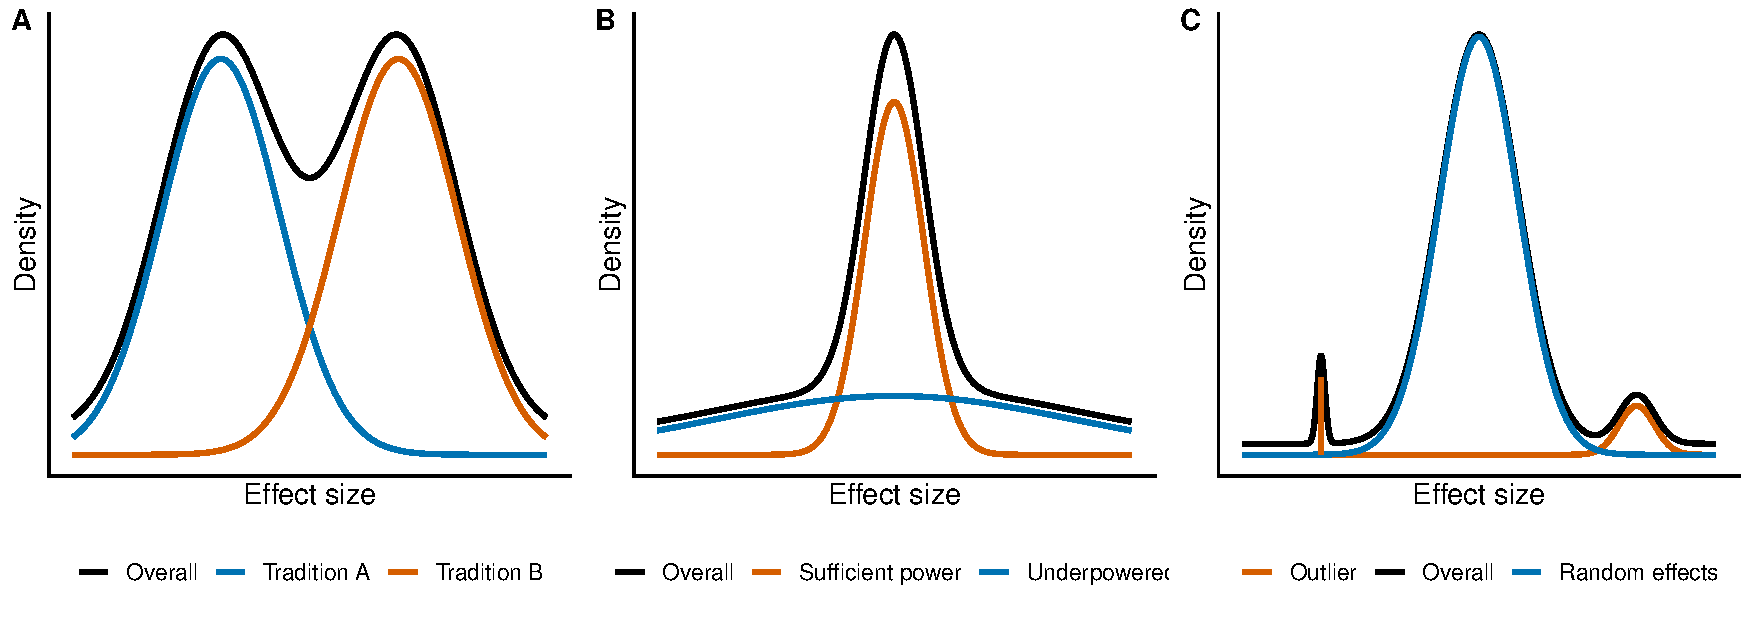
\includegraphics[keepaspectratio,alt={\label{fig:figmixexamples}Scenarios that give rise to mixture distributions: A) different research traditions resulting in distinct class means; B) underpowered studies resulting in distinct heterogeneity variances; C) a single outlier (left) or a cluster of outliers (right).}]{manuscript_files/figmixexamples.pdf}}
\caption{\label{fig:figmixexamples}Scenarios that give rise to mixture distributions: A) different research traditions resulting in distinct class means; B) underpowered studies resulting in distinct heterogeneity variances; C) a single outlier (left) or a cluster of outliers (right).}
\end{figure}

If a researcher is unaware of these systematic differences between effect sizes, they might conduct a meta-analysis of the effect sizes, ignoring these moderators.
A random-effects meta-analysis of all effect sizes would yield an unrepresentative pooled effect size: the average effect is exactly in the middle of both research traditions, and thus representative of neither.
Moverover, the estimated residual heterogeneity would be positively biased (inflated) by the differences between the two research traditions.

Even if the researcher had coded these moderators, they might still be practically prevented from accounting for them.
This moderator matrix has high multicolinearity: there is near-perfect overlap between the values of different moderators.
Including multicolinear moderators in a meta-regression makes it difficult to estimate each moderator's unique effect on effect size, resulting in unstable coefficient estimates, inflated standard errors, and poorly interpretable results (Steel \& Kammeyer-Mueller, 2002).
Thus, even if we had measured these systematic sources of heterogeneity, we might run into practical problems when trying to control for them.

As a second thought experiment, consider the presence of outliers in a meta-analytic dataset (example from Beath, 2014).
For example, imagine that a scholar has, for many years, asked undergraduate students to conduct pilot studies of a particular effect.
These pilot studies have small sample sizes, and thus show substantial variability in effect sizes.
Then, the researcher obtains funding to conduct a series of sufficiently powered experiments.
Not wanting students' work to go to waste, the researcher publishes a meta-analysis of all studies.
The distribution of effects will look like Figure \ref{fig:figmixexamples}B.
Note that the tails of the overall distribution are inflated by the presence of the underpowered studies.
In a random-effects meta-analysis, the estimated residual heterogeneity will be positively biased.

Finally, consider publication bias: the fact that significant findings are more likely to get published, leading to an overrepresentation of false-positive effect sizes in the literature.
It is plausible that phenomena exist whose true effect is zero, despite the existence of some (many) studies that report significant non-zero effects - purely due to publication bias (Collaboration, 2015).
Open science advocates have been advocating for changes to the publication culture that make it easier to publish null results (Lakens, Mesquida, Rasti, \& Ditroilo, 2024).
If we assume that both publication processes operate in parallel, the observed distribution of effect sizes in a field would be a mixture of two underlying distributions:
one centered around zero, reflecting studies that are published for their open science practices,
and one centered around a non-zero value, reflecting studies that are published because of their significant findings.

While these are thought experiments - they are meant to evoke realistic aspects of the scientific (publication) culture,
and give readers cause to question the widely held assumption that effect sizes are always normally distributed.
Each scenario gives a reason for why, sometimes, one random-effects distribution is not enough.
In these cases and others, mixture models can be used to disentangle multiple underlying random-effects distributions.

For example, \ref{fig:figmixexamples}A calls for a two-class mixture model with free means and equal variances.
This allows us to tease apart the unique pooled effect sizes of the two research traditions.
Of course - an expert might assign each study to one tradition, and treat ``assigned tradition'' as a moderating variable.
However, this approach ignores measurement error in the coding of assigned tradition.
Note that the traditions are not perfectly distinct, and that some studies share similarities with both traditions.
A mixture model is a more elegant solution, as it allows each case to contribute to the estimation of both distributions - and thus, ambiguous studies that resemble both traditions will contribute to both distributions.
This also resolved the aforementioned multicolinearity problem.

Figure \ref{fig:figmixexamples}B illustrates a two-class mixture model with equal means and free variances.
Such a model would tease apart the residual heterogeneity of the sufficiently powered studies from that of the underpowered studies.
The underpowered-class captures some of the heavy tails from the overall distribution,
thus enabling more powerful inference for the overall effect in the sufficiently-powered class.
Finally, Figure \ref{fig:figmixexamples}C requires a three-class model.
The overall distribution will have a free mean and variance,
as will the small cluster of outliers in the right tail.
The single outlier in the left tail can have a class of its own, with mean equal to the observed value, and variance fixed to zero (because variance for one observation is undefined).

\subsubsection{Previous Applications of Mixture Models in Meta-Analysis}\label{previous-applications-of-mixture-models-in-meta-analysis}

The present study is emphatically not the first to introduce mixture models in meta-analysis.
Prior work has demonstrated their usefulness for addressing several methodological challenges.

One such application is the use of mixture models for moderator analysis.
Different approaches have been taken; for example, some authors have used mixture models to dichotomize the moderator matrix, and use predicted class membership in meta-regression (Graefe, 2025).
This way, several study quality characteristics could be reduced to a single binary study quality indicator (high versus low), which could increase power to detect a moderator effect.
In this context, moderators are assumed to be measured without sampling error, and thus, the regular mixture model can be used.
Other authors have taken the inverse approach, performing mixture modeling on the effect sizes and then predicting class membership, rather than effect size value, in moderator analysis to increase statistical power (Zhang, Wang, \& Xu, 2022).
Apparently, these authors also use a random-effects mixture model, because the sampling variances are mentioned (p.~378).
However, the focus of the paper is moderator analysis and
the authors provide little detail on the mixture model implementation (``we treat the mixture decomposition algorithm as a black box'', p.~378).
The present paper introduces a more general random-effects mixture meta-analysis framework,
which can also be extended to moderator analysis via the weighted BCH approach (Bolck, Croon, \& Hagenaars, 2004), or via pseudo-class draws (Wang, Hendricks Brown, \& Bandeen-Roche, 2005), both implemented in \texttt{tidySEM} (C. J. Van Lissa et al., 2024).

Another study described the use of random-effects mixture modeling to perform robust meta-analysis (Beath, 2014).
This approach is suitable for scenarios like Figure \ref{fig:figmixexamples}B,
where the mixture distribution has heavy tails due to the presence of outliers.
It estimates two latent classes with a common mean and free variances.
Thus, one class can have a large variance and capture the outliers, while the other class offers less biased estimation of residual heterogeneity and more powerful inference for the pooled effect.
This method is implemented in the R-package \texttt{metaplus},
but as it is limited to 2-class models with equal means and free variances,
it is a special case of the more general framework introduced in this paper.

Other applications of meta-analytic mixture models have been developed in the context of diagnostic tests, to summarize tests' sensitivity and specificity across studies, and construct aggregate receiver operating characteristic curves (Eusebi, Reitsma, \& Vermunt, 2014; Schlattmann, Verba, Dewey, \& Walther, 2015).
One of these approaches models these test characteristics as discrete random effects, taking into account sampling variance but not residual heterogeneity within classes (Schlattmann et al., 2015).
While this method is implemented in an R-package, it has been removed from CRAN, and we were not able to compile an archived version to compare its performance to our method.
The other approach assumes binomial sampling distributions, which precludes its application to normal mixture models Eusebi et al. (2014){]}.
Moreover, it is only implemented in closed-source commercial software.
Importantly, these methods are designed for bivariate diagnostic accuracy outcomes rather than conventional univariate meta-analysis of continuous effect-size estimates with known sampling variances, which is the focus of the present study.

The research discussed here lays the foundation for the present work,
but differs in its intended applications, distributional assumptions, and generality.
We introduce \texttt{metamixture}, an open-source implementation of univariate random-effects mixture meta-analysis that accommodates class-specific or constrained mean effects and residual heterogeneity, while accounting for study-specific sampling variances.
Building on \texttt{OpenMx}, this implementation allows further model customization and extension, auxiliary analysis of predictors and moderators of class membership,
and use of existing tools for reporting and visualization, like \texttt{tidySEM}.
We evaluate the performance of these models in a simulation study, focusing on parameter recovery, confidence interval coverage, convergence, and the identification of the number of latent classes.

\subsubsection{Statistical Model}\label{statistical-model}

Finite mixture models represent the observed data distribution as a mixture of multiple underlying distributions.
Each observation has a probability of belonging to one of \(k\) latent classes;
the term ``finite'' implies that the number of components is known or fixed.
Each class, in turn, is defined by several parameters.
For continuous variables, these are often means \(\mu_{1 \ldots k}\) and variances \(\sigma^2_{1 \ldots k}\).
The overall distribution is a mixture of the class distributions, and each class contributes to the extent determined by the mixing proportion \(\pi_k\).
A class with a high mixing proportion contributes more to the overall distribution than one with a low mixing proportion.

Unlike mixture models for individual participant data, random-effects mixture models must account for sampling variance.
In the conventional random effects model, the observed sampling variance is treated as known to construct a weighted likelihood.
This model describes a single normal distribution of true effects, with its two parameters \(\mu\), the overall mean effect, and \(\tau^2\), the between-study variance or heterogeneity.
If we have coded observed effect sizes \(y_i\) and their sampling variances \(v_i\) from \(i \in 1 \ldots n\) studies, this model is:

\begin{equation}
y_i \sim \mathcal{N}(\mu,v_i+\tau^2)
\end{equation}

Note that the variance of individual effect sizes is composed of two parts: the residual heterogeneity \(\tau^2\), and individual sampling variance \(v_i\), which is treated as known.
When fitting this model to data, a (restricted) maximum likelihood estimator can be used to maximize the sum of the log-likelihood of individual observations, assuming a normal probability density \(\phi\):

\begin{equation}
\ell(\mu, \tau^2) = \sum_{i=1}^{n} \log \phi(y_i; \mu, v_i +\tau^2)
\end{equation}

We can extend this model to a finite mixture model for \(K\) latent classes.
Let \(C_i\) denote the unobserved class membership of observation \(i\).
The marginal density of each observed effect size is a weighted sum of class-specific normal densities, where the weights are determined by the mixing proportions \(\boldsymbol{\pi} = \pi_{1 \ldots K-1}\):
the proportion of the sample that belongs to each class.
Aside from these mixing proportions, the other model parameters are class-specific pooled effects and heterogeneities, \(\boldsymbol{\mu} = \mu_{1 \ldots K}\) and \(\boldsymbol{\tau^2} = \tau^2_{1 \ldots K}\).
Note that it is not necessary to estimate all \(K\) mixing proportions, because proportions sum to 1; one mixing proportion is given by taking 1 minus the sum of all others.
A \(K\)-class model thus has \(p=K+K+(K-1)=3K-1\) free parameters.

\begin{equation}
\ell(\boldsymbol{\pi}, \boldsymbol{\mu}, \boldsymbol{\tau}^2) =
\sum_{i=1}^{n}
\log
\left[\sum_{k=1}^{K} \pi_k \phi(y_i; \mu_k, v_i + \tau_k^2) \right]
\end{equation}

\subsubsection{Estimation}\label{estimation}

Estimation follows a three-stage procedure, based on the approach taken in the \texttt{tidySEM} R-package (C. J. Van Lissa et al., 2024).
This method should efficiently converge to global solutions while actively avoiding local solutions.
First, the sample is divided into \(K\) clusters by applying k-means clustering to the observed effect sizes (Hartigan \& Wong, 1979)\footnote{When class means are constrained to equality, the clustering is applied to the residuals instead.}.
Starting values for the class-specific mean effect sizes and residual heterogeneity variances are computed for each cluster using the DL-estimator (DerSimonian \& Laird, 1986).
Initial class proportions are set to the cluster proportions.
Next, simulated annealing is used to explore the likelihood surface and search for a global optimum (Pervez \& Lee, 2015).
Unlike numerical optimization, which greedily approaches the closest maximum from the starting values,
simulated annealing occasionally accepts parameter changes that worsen model fit.
This is useful, because mixture models' likelihood tends to have many local optima where a greedy algorithm could get stuck.
Simulated annealing actively escapes local optima and explores alternative solutions.
Over time, worsening moves become less likely, encouraging convergence toward a promising solution.
The final likelihood from simulated annealing is further refined using numerical optimization.

Simulated annealing is efficient compared to the brute-force approach of using many random starting values - but neither method is guaranteed to find the global optimum solution.
If convergence is not obtained,
20 sets of random starting values are evaluated in an attempt to find a better solution.
Once the model has converged, standard errors and profile-likelihood confidence intervals are calculated.

\subsubsection{Class Enumeration}\label{class-enumeration}

When the number of classes is known on theoretical grounds, it is sufficient to estimate the \(K\)-class model, and optionally, to test the hypotheses that \(K\)-classes suffice (C. J. Van Lissa et al., 2024).
However, mixture modeling is also used for exploratory analyses of heterogeneity.
In these cases, \(K\) is determined in a data-driven manner.
Two well-established approaches to class enumeration are information theoretical methods, and likelihood ratio tests.
Information theoretical methods select the model with the lowest value on a statistic that balances model fit and complexity, by adding a complexity penalty to the minus two log-likelihood.
Examples include the Akaike Information Criterion (AIC, Akaike, 1974), Bayesian Information Criterion (BIC, Schwarz, 1978), or Integrated Completed Likelihood (Biernacki, Celeux, \& Govaert, 2000), where the latter is unique in penalizing poor class separation as well.
A limitation of these methods is that they do not offer significance tests.
Likelihood ratio tests do offer such tests, but are generally problematic for mixture models because when comparing a \(K-1\) and \(K\)-class model, the \(K-1\) model's parameters for one class are set to zero, which is on the boundary of the parameter space of the \(K\)-class model.
The Bootstrapped Likelihood Ratio Test is an exception (BLRT, McLachlan, 1987).
However, its major limitation is that it re-estimates all models on all bootstrap samples (i.e., 100 or 1000 times or more),
which is computationally very expensive.

A recently introduced approach is Predictive Model Comparison (PMC).
Based on the ``lazy bootstrap'', PMC repeatedly simulates data from each fitted model and evaluates how closely the simulated data distributions resemble the observed data (Kollenburg, Mulder, \& Vermunt, 2018).
For univariate data like effect sizes, one could use a metric that captures how ``surprising'' the simulated data is, in the context of the empirical observed data distribution (Shannon, 1948).
The surprisal statistic is given as the sum of negative log probability densities of the observed data in the (estimated) density distribution of a simulated dataset.
Lower values indicate that the the observed data have greater probability density in the simulated data distribution, which means it is a good approximation of the observed data distribution.
Repeating the simulation yields a distribution of surprisal statistics,
from which confidence intervals for differences in mean surprisal between models can be constructed.
A model with \(K\) classes is preferred over a model with \(K-1\) classes when the confidence interval indicates a reduction in expected surprisal.

Another potential approach is to use cross-validation (Hastie, Tibshirani, \& Friedman, 2009).
First, observed effect sizes are randomly split into multiple subsets.
Each candidate model is fitted on effect sizes from all subsets except one, and the fitted model's predictive performance is evaluated on the one held-out subset.
The aforementioned surprisal statistic can again be used to evaluate performance, with a key distinction that the likelihood of the held-out effect sizes can be directly evaluated with respect to the cross-validated model's parameters, rather then the simulated data density.
Surprisal scores are summed across subsets.
The model with the lowest value has the best out-of-sample predictive performance, and is selected.
While this method also requires re-fitting models, it only estimates each model a few times, compared to BLRT's 100s or 1000s of times.
At present, the best-performing class enumeration methods for individual participant data appear to be the BIC and BLRT (see C. J. Van Lissa et al., 2024).
However, their performance for random-effects mixture meta-analysis is unknown.

\subsubsection{The Present Study}\label{the-present-study}

We introduce and validate a method for estimating random-effects mixture meta-analysis models that accommodates known, study-specific sampling variances.
In a comprehensive simulation study, we examine the method's parameter bias, confidence interval coverage, and the performance of different approaches to class enumeration.

\subsection{Study 1: Validation of Random-Effects Mixture Meta-Analysis}\label{study-1-validation-of-random-effects-mixture-meta-analysis}

We used a factorial design with 100 replications for each unique combination of conditions.
The true number of classes was \(K \in (1, 2, 3)\).
The difference in true means between classes was \(\Delta_\mu = (1, 2, 3)\).
Because residual heterogeneity was fixed at \(1\), these values can be interpreted as the number of standard deviations difference between successive class means.
Class imbalance was manipulated as the ratio between the size of the first class and the rest, where the first class was \(p_{\text{ratio}} \in (1, 1.5, 2)\) times as large as the other classes.
Other simulation parameters were based on observed properties of 705 empirical meta-analyses (Van Erp, Verhagen, Grasman, \& Wagenmakers, 2017).
We manipulated the number of true effect sizes, \(n \in (20, 50, 100, 300)\),
Note that 20 observations is already a substantial sample in meta-analysis, but mixture models have many parameters, so a reasonable sample size is required.
As a 4-class model has 11 parameters, a sample of 20 effect sizes gives fewer than two observations per parameter.
Individual effect sizes' sampling variance was drawn from a uniform distribution between \(0\) and \(v_{\text{max}} \in (.001, .01, .1)\).
Note that, for one true class, \(\Delta_\mu\) and \(p_{\text{ratio}}\) are meaningless and were collapsed to 0 and 1, respectively.
For a 2-class model with equal mixing proportions and residual heterogeneity up to \(.01\), the population mixture distribution and the empirical distribution of a sample of 100 effect sizes is shown in Figure \ref{fig:figsim}.
Note that the classes are difficult to distinquish in the empirical distribution,
except when \(\Delta_\mu = 3\).

\begin{figure}
\centering
\pandocbounded{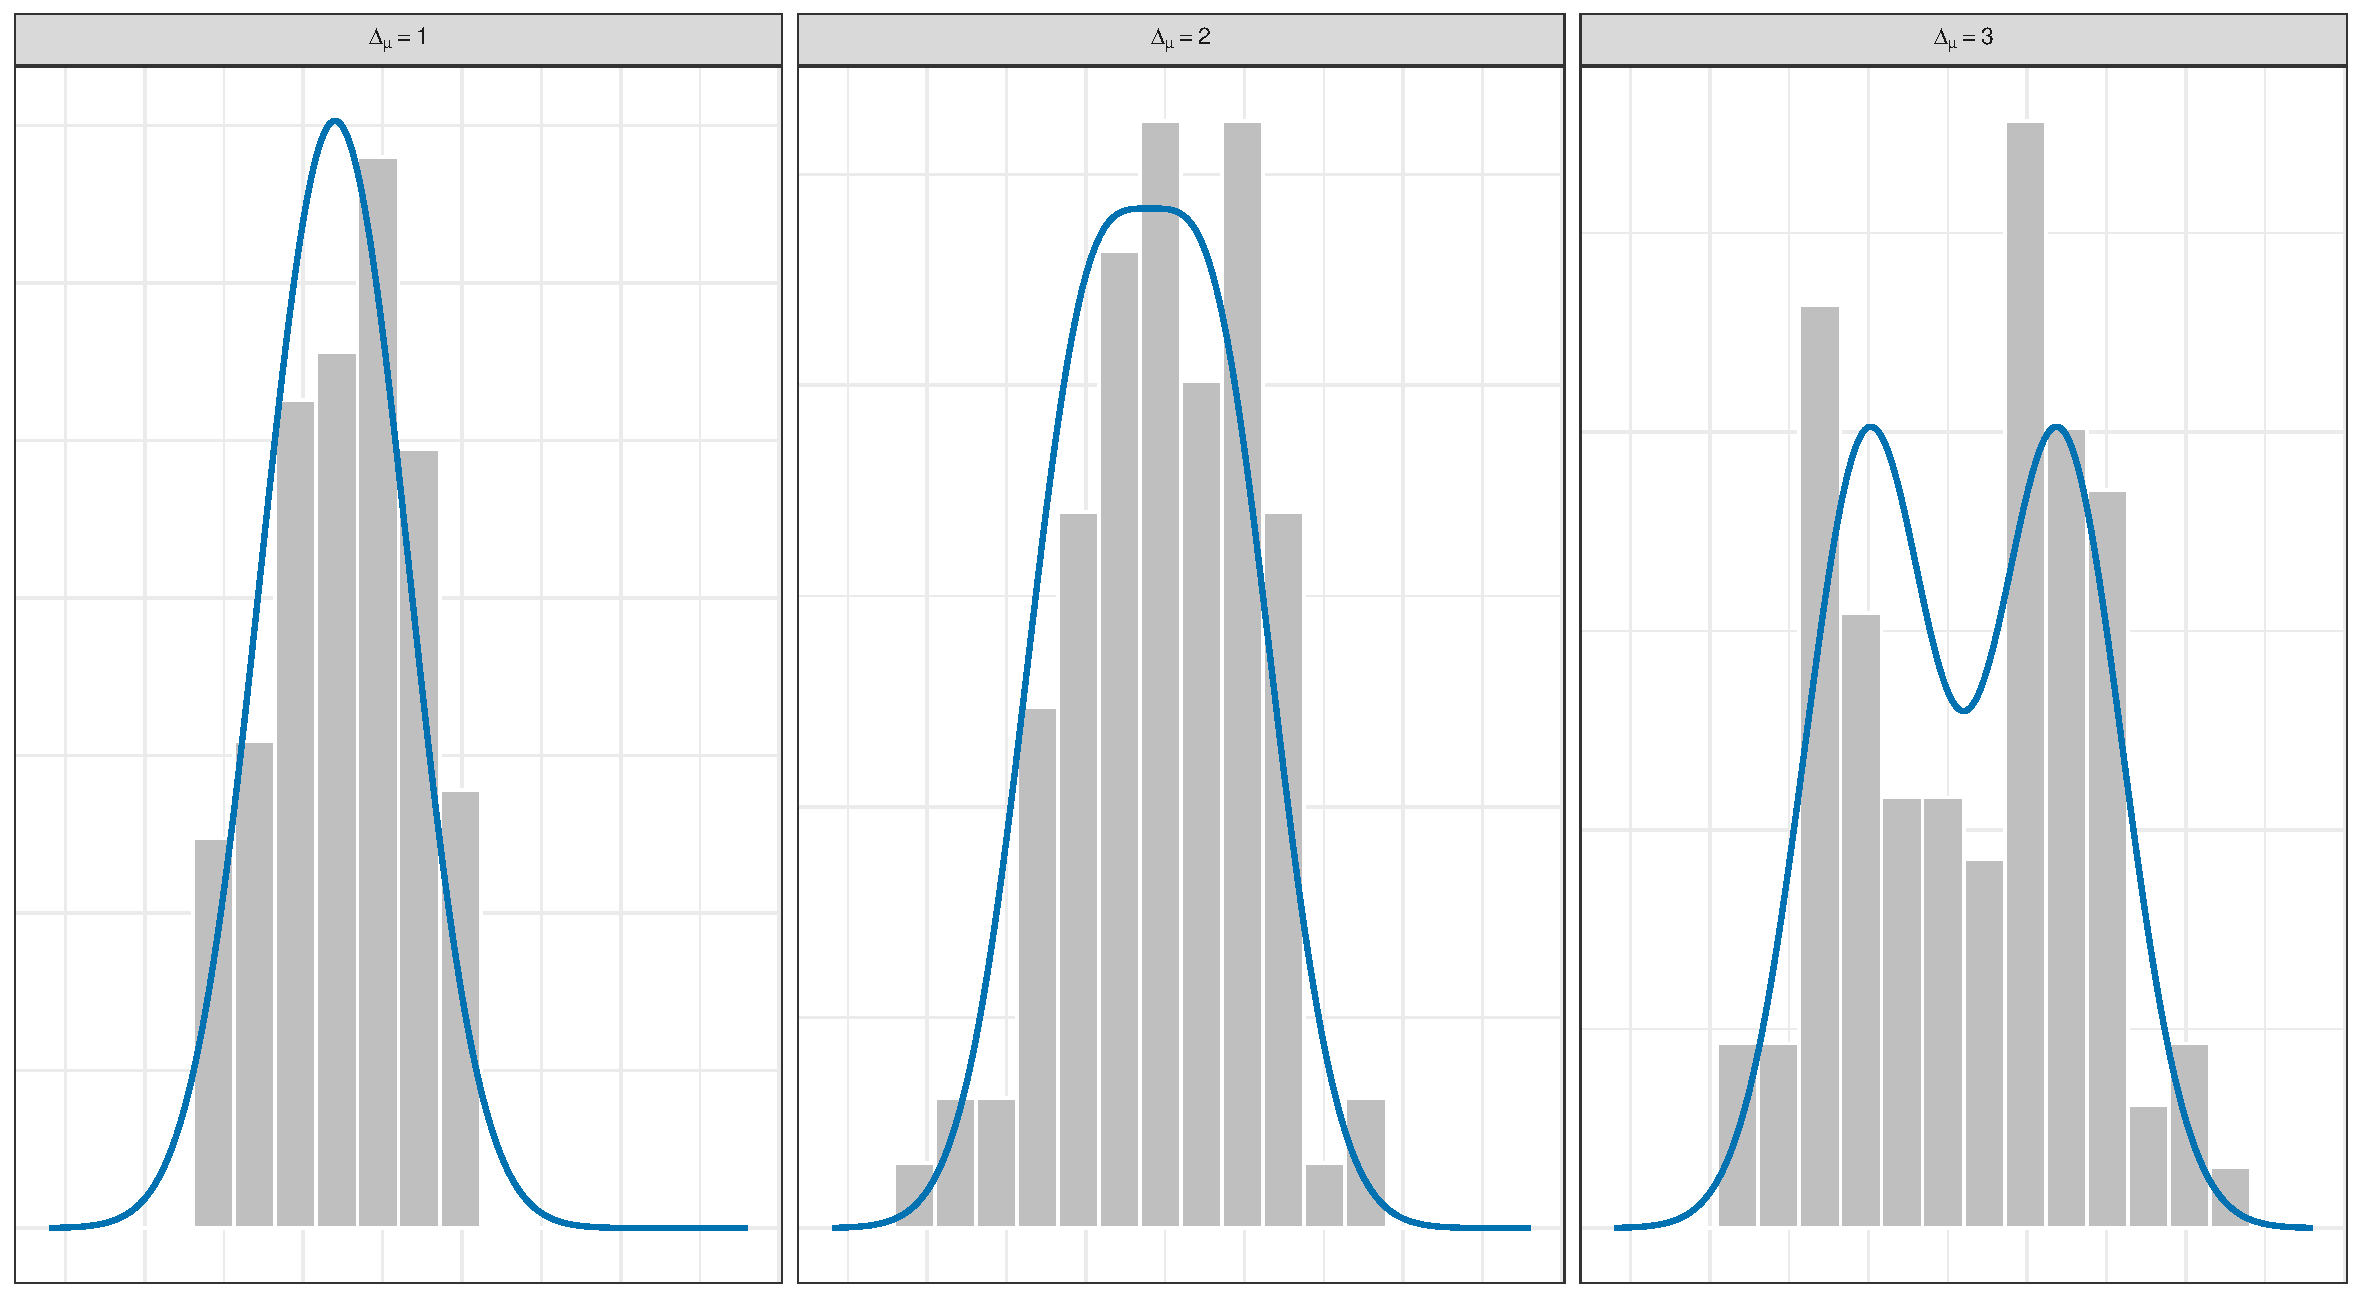
\includegraphics[keepaspectratio,alt={\label{fig:figsim}Population mixture distribution (blue) and histogram of empirical distribution (gray histogram) of 100 observations.}]{manuscript_files/figsim.pdf}}
\caption{\label{fig:figsim}Population mixture distribution (blue) and histogram of empirical distribution (gray histogram) of 100 observations.}
\end{figure}

\subsection{Results}\label{results}

We used the Workflow for Open Reproducible Code in Science (WORCS, Caspar J. Van Lissa et al., 2021) to render all analysis code reproducible.
The research archive is available at \href{}{MASKED FOR REVIEW}.
The simulation code can be adapted to examine other scenarios not covered in the present study, or to perform power analysis.

\subsubsection{Bias}\label{bias}

Table \ref{tab:tabesbias} shows effect sizes (partial \(\eta^2\)) of the simulation conditions on signed and absolute bias.
Note that these effect sizes are only interpretable within the range of values examined in this simulation study; expanding the range will increase the effect sizes of relevant factors.
The estimates of \(\mu\) were unbiased on average, and signed bias was not affected by any design factors.
However, absolute bias decreased with increasing sample size and effect size, and increased with increasing number of classes.
The estimates of \(\tau^2\) were negatively biased on average, and signed- and absolute bias were similarly affected by design factors.
Specifically, bias in \(\tau^2\) decreased with increasing sample size and effect size, and increased with increasing number of classes.
Finally, estimates of \(\pi\) were nearly unbiased on average.
Signed bias in \(\pi\) decreased slightly with increasing effect size.
Absolute bias in \(\pi\) was highly sensitive to effect size; thus, there were larger discrepancies at smaller effect sizes.
Other effects for \(\pi\) were near-zero.

\begin{table}[tbp]

\begin{center}
\begin{threeparttable}

\caption{\label{tab:tabesbias}Effect size (partial $\eta^2$) of simulation conditions on bias.}

\begin{tabular}{lllllll}
\toprule
type & \multicolumn{1}{c}{parameter} & \multicolumn{1}{c}{C} & \multicolumn{1}{c}{$\Delta_{\mu}$} & \multicolumn{1}{c}{K} & \multicolumn{1}{c}{$p_{\text{ratio}}$} & \multicolumn{1}{c}{$v_i$}\\
\midrule
Bias & $\mu$ & 0.00 & 0.00 & 0.00 & 0.00 & 0.00\\
Bias & $\tau^2$ & 0.04 & 0.18 & 0.13 & 0.00 & 0.00\\
Bias & $\pi$ & 0.01 & 0.03 & 0.00 & 0.01 & 0.00\\
Absolute bias & $\mu$ & 0.05 & 0.08 & 0.09 & 0.01 & 0.00\\
Absolute bias & $\tau^2$ & 0.08 & 0.09 & 0.20 & 0.00 & 0.00\\
Absolute bias & $\pi$ & 0.01 & 0.22 & 0.02 & 0.00 & 0.00\\
\bottomrule
\end{tabular}

\end{threeparttable}
\end{center}

\end{table}

\begin{figure}
\centering
\pandocbounded{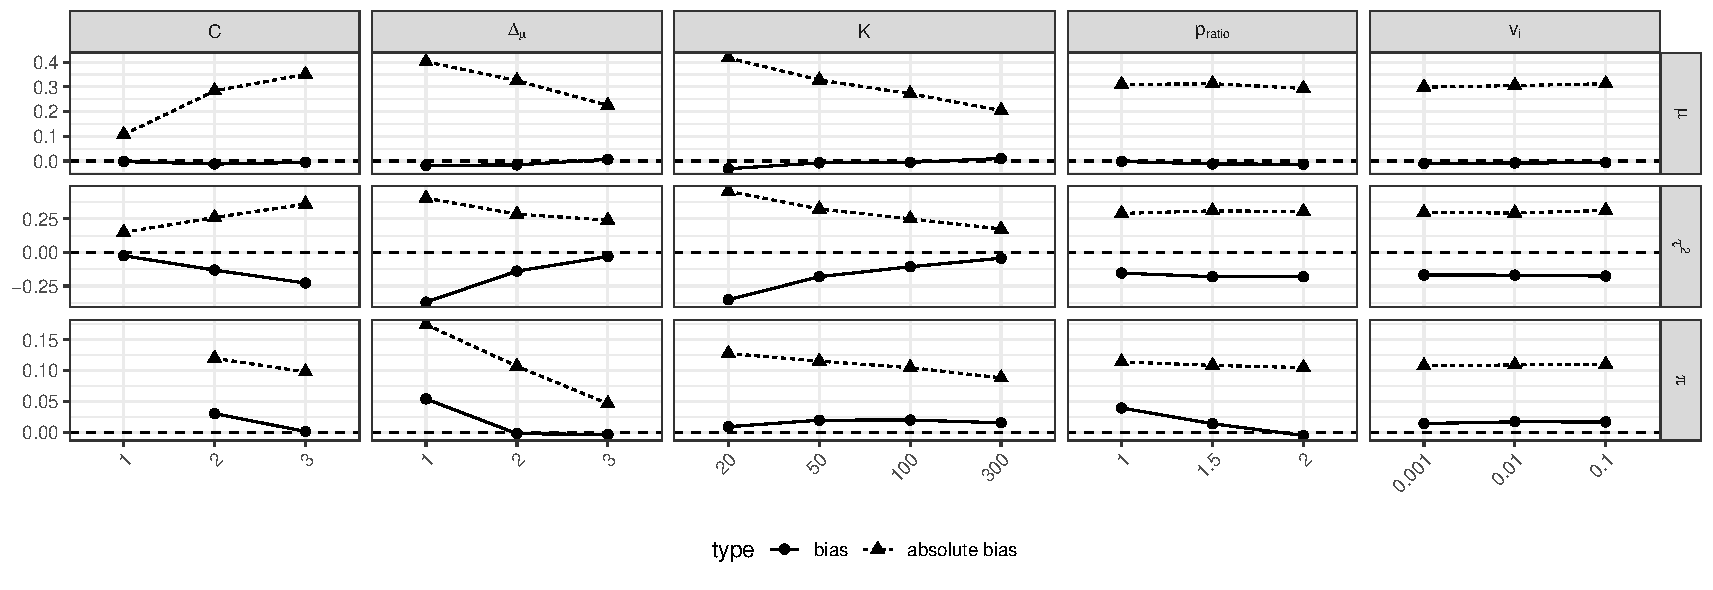
\includegraphics[keepaspectratio,alt={\label{fig:figbias}Marginal effects of simulation conditions on parameter estimate bias.}]{manuscript_files/output/plot_bias.pdf}}
\caption{\label{fig:figbias}Marginal effects of simulation conditions on parameter estimate bias.}
\end{figure}

\subsubsection{Confidence Interval Coverage}\label{confidence-interval-coverage}

Table \ref{tab:tabcov} shows effect sizes of the simulation conditions on CI coverage, and Figure \ref{fig:figcov} shows their marginal effects.
On average, CI coverage was below nominal levels for \(\mu\) and \(\pi\) in all conditions, except for \(\pi\) when effect size was at its maximum value of \(3\).
CI coverage was at its ceiling for \(\tau^2\) across all conditions.
CI coverage of \(\mu\) increased with increasing effect size, and decreased with an increasing number of classes.
Coverage of \(\pi\) also increased with increasing effect size.

\begin{table}[tbp]

\begin{center}
\begin{threeparttable}

\caption{\label{tab:tabcov}Effect size (partial $\eta^2$) of simulation conditions on confidence interval coverage.}

\begin{tabular}{llllll}
\toprule
parameter & \multicolumn{1}{c}{C} & \multicolumn{1}{c}{$\Delta_{\mu}$} & \multicolumn{1}{c}{K} & \multicolumn{1}{c}{$p_{\text{ratio}}$} & \multicolumn{1}{c}{$v_i$}\\
\midrule
$\mu$ & 0.01 & 0.08 & 0.00 & 0.00 & 0.00\\
$\tau^2$ & 0.00 & 0.00 & 0.00 & 0.00 & 0.00\\
$\pi$ & 0.00 & 0.09 & 0.00 & 0.00 & 0.00\\
\bottomrule
\end{tabular}

\end{threeparttable}
\end{center}

\end{table}

\begin{figure}
\centering
\pandocbounded{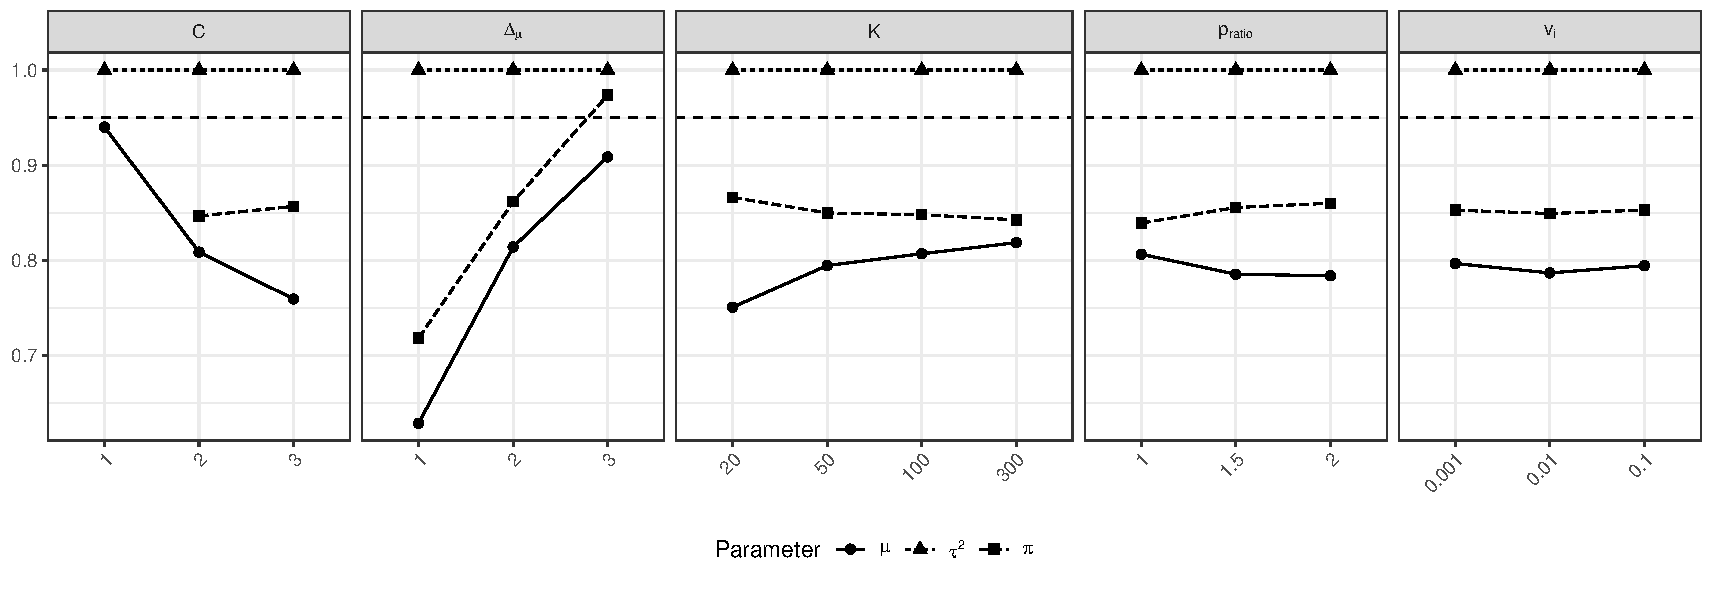
\includegraphics[keepaspectratio,alt={\label{fig:figcov}Marginal effects of simulation conditions on mean confidence interval coverage.}]{manuscript_files/output/plot_cov2.pdf}}
\caption{\label{fig:figcov}Marginal effects of simulation conditions on mean confidence interval coverage.}
\end{figure}

\subsubsection{Class Enumeration}\label{class-enumeration-1}

On average, the class enumeration metrics all performed at near-chance levels.
For 1-4 class models, randomly choosing a solution would yield 25\% performance.
The best-performing algorithm was AIC (p = 0.34), followed by PMC (p= 0.34), CV (p= 0.28), BIC (p= 0.24), and ICL (p = 0.08).

Table \ref{tab:tabenum} shows effect sizes, and \ref{fig:figenum} shows the marginal effects of simulation conditions on class enumeration performance.
AIC, BIC, and CV were most influenced by effect size (greater effect sizes resulted in better performance), followed by number of classes (more classes resulted in worse performance), and sample size (larger samples resulted in better performance).
ICL was most influenced by number of classes.
PMC was largely invariant to simulation conditions.
The poor performance of these algorithms was mostly due to underfitting; overfitting barely occurred.

\begin{table}[tbp]

\begin{center}
\begin{threeparttable}

\caption{\label{tab:tabenum}Effect size (partial $\eta^2$) of simulation conditions on class enumeration accuracy (selected solution equals true number of classes).}

\begin{tabular}{llllll}
\toprule
parameter & \multicolumn{1}{c}{C} & \multicolumn{1}{c}{$\Delta_{\mu}$} & \multicolumn{1}{c}{K} & \multicolumn{1}{c}{$p_{\text{ratio}}$} & \multicolumn{1}{c}{$v_i$}\\
\midrule
aic & 0.08 & 0.20 & 0.05 & 0.00 & 0.00\\
bic & 0.25 & 0.31 & 0.07 & 0.00 & 0.00\\
cv & 0.12 & 0.14 & 0.05 & 0.00 & 0.00\\
icl & 0.61 & 0.03 & 0.02 & 0.00 & 0.00\\
pmc & 0.00 & 0.05 & 0.01 & 0.00 & 0.00\\
\bottomrule
\end{tabular}

\end{threeparttable}
\end{center}

\end{table}

\begin{figure}
\centering
\pandocbounded{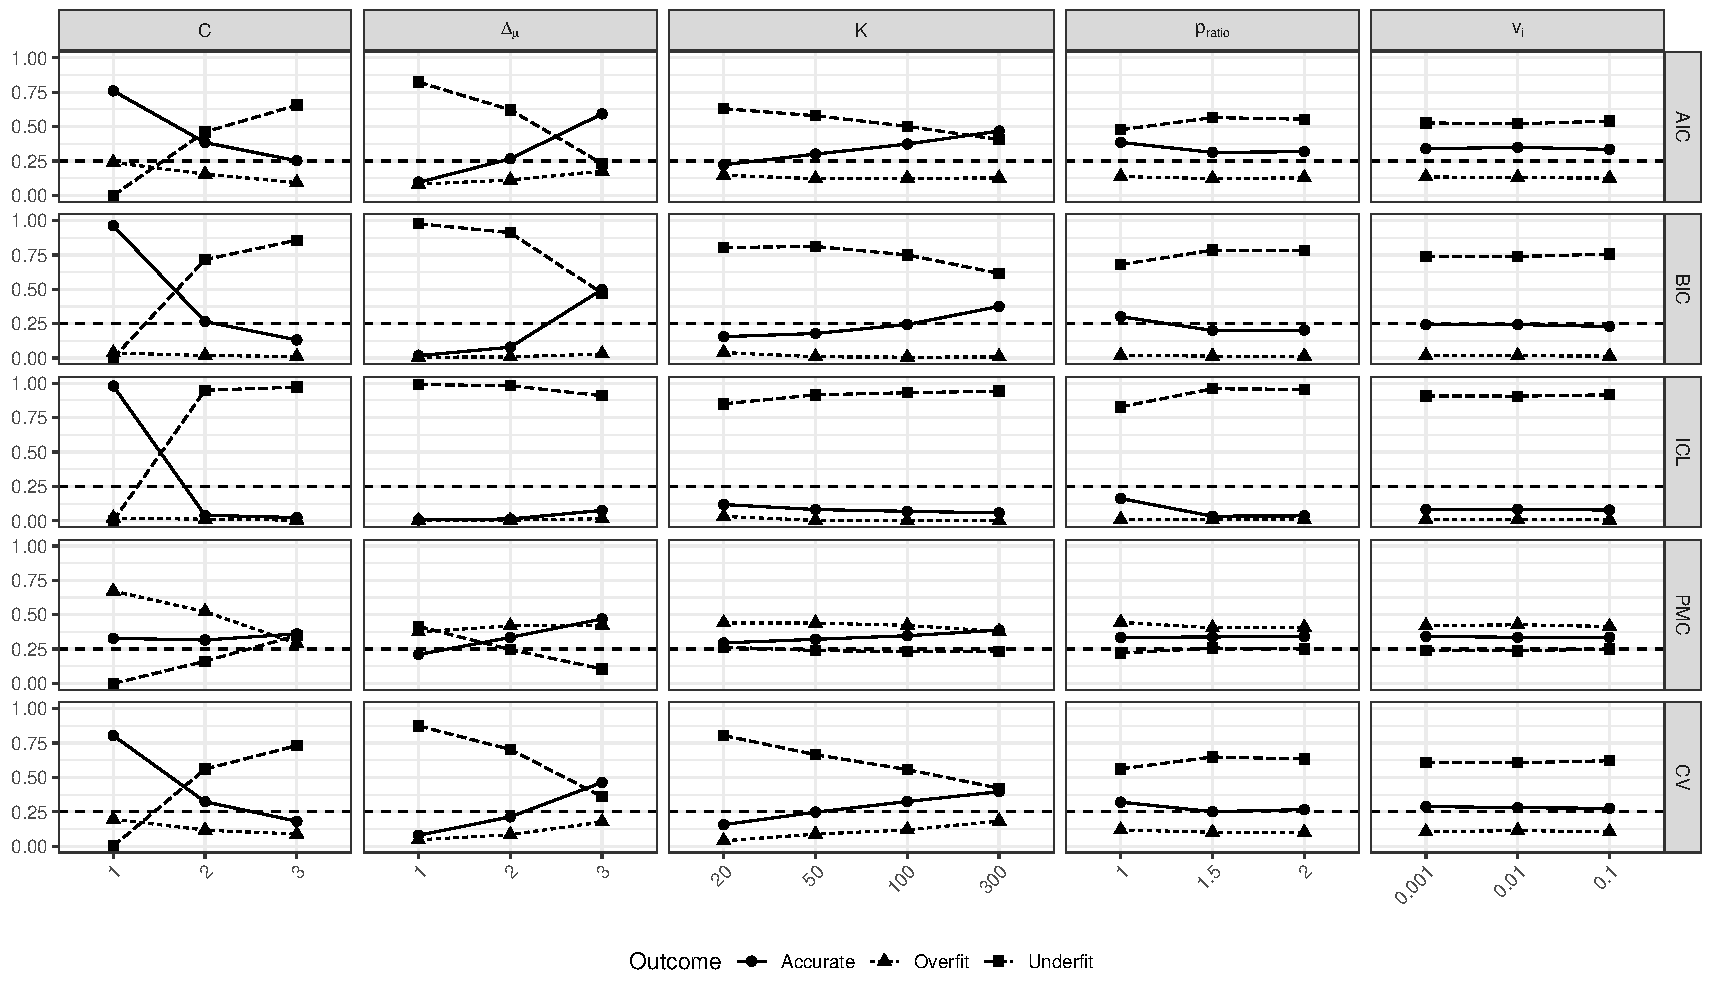
\includegraphics[keepaspectratio,alt={\label{fig:figenum}Marginal effects of simulation conditions on class enumeration.}]{manuscript_files/output/plot_enum.pdf}}
\caption{\label{fig:figenum}Marginal effects of simulation conditions on class enumeration.}
\end{figure}

\subsection{\texorpdfstring{Study 2: Comparison to \texttt{metaplus}}{Study 2: Comparison to metaplus}}\label{study-2-comparison-to-metaplus}

Since the \texttt{metaplus} R-package offers functionality that partly overlaps with the general random-effects mixture meta-analysis framework introduced here, we conducted a second, smaller study to compare the two methods.
The \texttt{metaplus} R-package exclusively estimate 2-class mixture models with a shared mean and distinct heterogeneity parameters.
We examined the convergence of both methods,
time required to run the analysis,
bias in parameter estimates and proportion of cases in which each algorithm outperformed the other in terms of parameter accuracy,
and covariance coverage.

Simulation parameters were chosen to favor \texttt{metaplus}:
We fixed the true number of classes at \(K = 2\) with no mean difference and distinct heterogeneity parameters between classes.
As before, heterogeneity in the first class was fixed at 1,
and heterogeneity in the second class was either \(\tau^2_{\text{ratio}} \in (2, 4, 6)\).
The number of replications, sample sizes, class size ratios, sampling variances, and number of replications were identical to Study 1,
yielding 15600 simulation runs.

\subsection{Results}\label{results-1}

\begin{table}[tbp]

\begin{center}
\begin{threeparttable}

\caption{\label{tab:tabmetaplus}Results of Study 2}

\begin{tabular}{llllllllll}
\toprule
method & \multicolumn{1}{c}{$MAE_{\mu}$} & \multicolumn{1}{c}{$MAE_{\tau^2}$} & \multicolumn{1}{c}{$MAE_{\pi}$} & \multicolumn{1}{c}{$Acc_{\mu}$} & \multicolumn{1}{c}{$Acc_{\tau^2}$} & \multicolumn{1}{c}{$Acc_{\pi}$} & \multicolumn{1}{c}{$CC_{\mu}$} & \multicolumn{1}{c}{$CC_{\tau^2}$} & \multicolumn{1}{c}{$CC_{\pi}$}\\
\midrule
remix & 0.15 & 0.45 & 0.24 & 0.34 & 0.54 & 0.51 & 0.91 & 0.69 & 0.74\\
metaplus & 0.18 & 0.46 & 0.23 & 0.66 & 0.46 & 0.49 & 0.92 &  & \\
\bottomrule
\addlinespace
\end{tabular}

\begin{tablenotes}[para]
\normalsize{\textit{Note.} Mean absolute error (MAE), proportion of replications in which each algorithm was more accurate (lower bias) than the other (Acc), and Confidence interval coverage (CC).}
\end{tablenotes}

\end{threeparttable}
\end{center}

\end{table}

The \texttt{metaplus} algorithm converged in all iterations, whereas \texttt{remix} converged in \(87.50\)\% of cases.
This difference might be due to the fact that \texttt{metaplus} uses random starting values by default, whereas \texttt{remix} does not.
To aid convergence, it is possible to run \texttt{random\_starts()} on a non-converged \texttt{remix} object.
The median runtime of \texttt{metaplus} analyses was \(14.91\) seconds, compared to \texttt{remix}' \(0.53\) seconds.
Thus, \texttt{remix} was about \(28\) times faster to run.

As shown in Table \ref{tab:tabmetaplus}, the mean absolute error (bias) of \texttt{remix} was lower for the pooled effect \(\mu\) and residual heterogeneity \(\tau^2\), but slightly higher for the mixing proportion \(\pi\), when compared to \texttt{metaplus}.
However, this pattern of results was reversed when examining the mean relative accuracy (which algorithm has lower bias within each iteration);
here, \texttt{remix} performed worse for \(\mu\), and better for \(\tau^2\) and \(\pi\).
This suggests that, although \texttt{metaplus} more often gives the less biased estimate for \(\mu\), when it's wrong, it tends to have larger errors than \texttt{remix}.

In terms of confidence interval (CI) coverage, we see a \(1\)\% difference in coverage for \(\mu\), but both algorithms' coverage is below the nominal level of \(95\)\%.
This issue is exacerbated for \texttt{remix}' CI coverage for \(\tau^2\) and \(\pi\).
As \texttt{metaplus} returned all missing values for the CIs of \(\tau^2\) and \(\pi\), we cannot evaluate its performance.

\subsection{Discussion}\label{discussion}

Interpret findings

Discuss implications

\begin{itemize}
\item
  A single \(\tau^2\) may obscure distinct distributional structures.
\item
  Mixture models offer a complementary perspective on unexplained heterogeneity.
\item
  Class-specific estimates may reveal patterns that a pooled effect and single heterogeneity estimate cannot adequately summarize.
\item
  Mixture modeling may guide subsequent moderator analyses by suggesting potential subgroup structure.
\end{itemize}

\subsubsection{Strengths}\label{strengths}

We implement this method in the \texttt{remix()} function of the \texttt{metamixture} package, with a backend in \texttt{OpenMx} - a flexible, customizable and extensible structural equation modeling framework.
Using \texttt{OpenMx} to estimate \texttt{remix()} models has several advantages.
First, \texttt{OpenMx} performs efficient optimization, and is very fast.
Second, it is a general-purpose structural equation modeling framework,
which means models can be fully customized (e.g., with equality constraints, starting values, auxiliary variables).
It provides standard errors and profile-likelihood confidence intervals out of the box,
and interfaces with many other packages for downstream analyses and tabulation and plotting of results (e.g., tidySEM, C. J. Van Lissa et al., 2024).

Emphasize flexibility rather than novelty of the underlying mixture distribution.

\begin{itemize}
\item
  Straightforward specification of location and scale mixtures.
\item
  Explicit incorporation of known sampling variances.
\item
  Equality constraints and alternative model structures.
\item
  Flexible optimization and likelihood-based inference.
\item
  Extensibility to more complex models.
\end{itemize}

\subsubsection{Limitations}\label{limitations}

\begin{itemize}
\item
  Weak identification with overlapping or very small components.
\item
  Dependence on sample size and class separation.
\item
  Local maxima and sensitivity to initialization.
\item
  Nonregular inference for boundary parameters and class enumeration.
\item
  Potential for interpreting distributional approximations as substantive classes.
\item
  Misspecification when true effects follow skewed, heavy-tailed, or continuously heterogeneous distributions rather than distinct latent classes.
\end{itemize}

\subsubsection{Recommendations for applied researchers}\label{recommendations-for-applied-researchers}

Develop practical guidance on when mixture modeling is useful, how many classes to consider, how to assess convergence, and how to interpret posterior classifications.

Recommend sensitivity analyses across model specifications and starting values, and caution against interpreting every additional class as a substantively distinct study population.

\subsubsection{Future directions}\label{future-directions}

\begin{itemize}
\item
  Mixture meta-regression incorporating observed moderators.
\item
  Multivariate and multilevel random-effects mixtures.
\item
  Alternative within-class distributions.
\item
  Bayesian estimation and uncertainty in class enumeration.
\item
  Extensions to dependent effect sizes.
\item
  More comprehensive simulation-based inference.
\end{itemize}

\subsection{Conclusion}\label{conclusion}

Reiterate that conventional random-effects meta-analysis models heterogeneity primarily through a single distribution, whereas finite mixture models offer a flexible way to investigate potentially more complex effect-size distributions.

The proposed OpenMx implementation aims to make this framework accessible, extensible, and amenable to systematic model comparison and likelihood-based inference. The simulation study will establish the conditions under which this added flexibility provides reliable estimates and useful insights, as well as the circumstances in which conventional approaches remain preferable.

Contributions:

\begin{enumerate}
\def\labelenumi{\arabic{enumi}.}
\item
  A unified modeling framework that accommodates location mixtures, scale mixtures, and location-scale mixtures while respecting known sampling variances.
\item
  A flexible OpenMx implementation that facilitates model constraints, likelihood-based inference, optimization, and extensions beyond standard univariate random-effects models.
\item
  A systematic simulation-based evaluation of when these models can reliably recover latent heterogeneity structures and when estimation, class enumeration, or inference becomes problematic.
\end{enumerate}

\newpage

\section{References}\label{references}

\protect\phantomsection\label{refs}
\begin{CSLReferences}{1}{0}
\bibitem[\citeproctext]{ref-akaikeNewLookStatistical1974}
Akaike, H. (1974). A new look at the statistical model identification. \emph{IEEE Transactions on Automatic Control}, \emph{19}(6), 716--723. \url{https://doi.org/10.1109/TAC.1974.1100705}

\bibitem[\citeproctext]{ref-beathFiniteMixtureMethod2014}
Beath, K. J. (2014). A finite mixture method for outlier detection and robustness in meta-analysis. \emph{Research Synthesis Methods}, \emph{5}(4), 285--293. \url{https://doi.org/10.1002/jrsm.1114}

\bibitem[\citeproctext]{ref-biernackiAssessingMixtureModel2000}
Biernacki, C., Celeux, G., \& Govaert, G. (2000). Assessing a mixture model for clustering with the integrated completed likelihood. \emph{IEEE Transactions on Pattern Analysis and Machine Intelligence}, \emph{22}(7), 719--725. \url{https://doi.org/10.1109/34.865189}

\bibitem[\citeproctext]{ref-bokerOpenMxOpenSource2011}
Boker, S., Neale, M., Maes, H., Wilde, M., Spiegel, M., Brick, T., \ldots{} Fox, J. (2011). {OpenMx}: {An Open Source Extended Structural Equation Modeling Framework}. \emph{Psychometrika}, \emph{76}(2), 306--317. \url{https://doi.org/10.1007/s11336-010-9200-6}

\bibitem[\citeproctext]{ref-bolckEstimatingLatentStructure2004}
Bolck, A., Croon, M., \& Hagenaars, J. (2004). Estimating {Latent Structure Models} with {Categorical Variables}: {One-Step Versus Three-Step Estimators}. \emph{Political Analysis}, \emph{12}(1), 3--27. \url{https://doi.org/10.1093/pan/mph001}

\bibitem[\citeproctext]{ref-collaborationEstimatingReproducibilityPsychological2015}
Collaboration, O. S. (2015). Estimating the reproducibility of psychological science. \emph{Science}, \emph{349}(6251). \url{https://doi.org/10.1126/science.aac4716}

\bibitem[\citeproctext]{ref-dersimonianMetaanalysisClinicalTrials1986}
DerSimonian, R., \& Laird, N. (1986). Meta-analysis in clinical trials. \emph{Controlled Clinical Trials}, \emph{7}(3), 177--188. \url{https://doi.org/10.1016/0197-2456(86)90046-2}

\bibitem[\citeproctext]{ref-eusebiLatentClassBivariate2014}
Eusebi, P., Reitsma, J. B., \& Vermunt, J. K. (2014). Latent class bivariate model for the meta-analysis of diagnostic test accuracy studies. \emph{BMC Medical Research Methodology}, \emph{14}(1), 88. \url{https://doi.org/10.1186/1471-2288-14-88}

\bibitem[\citeproctext]{ref-graefeApplicationFiniteMixture2025}
Graefe, B. E. (2025). \emph{Application of {Finite Mixture Modeling} in {Meta-Analysis} for {Evaluating Between-Study Heterogeneity} - {University} of {Miami}} (PhD thesis, University of Miami). University of Miami, Miami. Retrieved from \url{https://scholarship.miami.edu/esploro/outputs/doctoral/Application-of-Finite-Mixture-Modeling-in/991032699553802976?institution=01UOML_INST}

\bibitem[\citeproctext]{ref-hartiganAlgorithm136KMeans1979}
Hartigan, J. A., \& Wong, M. A. (1979). Algorithm {AS} 136: {A K-Means Clustering Algorithm}. \emph{Journal of the Royal Statistical Society. Series C (Applied Statistics)}, \emph{28}(1), 100--108. \url{https://doi.org/10.2307/2346830}

\bibitem[\citeproctext]{ref-hastieElementsStatisticalLearning2009}
Hastie, T., Tibshirani, R., \& Friedman, J. (2009). \emph{The elements of statistical learning: {Data} mining, inference, and prediction} (Second). New York: Springer.

\bibitem[\citeproctext]{ref-hedgesFixedRandomeffectsModels1998}
Hedges, L. V., \& Vevea, J. L. (1998). Fixed- and {Random}-effects {Models} in {Meta}-analysis. \emph{Psychological Methods}, \emph{3}(4), 486--504. Retrieved from \url{https://insights.ovid.com/psychological-methods/plmet/1998/12/000/fixed-random-effects-models-meta-analysis/6/00060744}

\bibitem[\citeproctext]{ref-kollenburgLazyBootstrapFast2018}
Kollenburg, G. H. van, Mulder, J., \& Vermunt, J. K. (2018, January 29). The {Lazy Bootstrap}. {A Fast Resampling Method} for {Evaluating Latent Class Model Fit}. \url{https://doi.org/10.48550/arXiv.1801.09519}

\bibitem[\citeproctext]{ref-lakensBenefitsPreregistrationRegistered2024}
Lakens, D., Mesquida, C., Rasti, S., \& Ditroilo, M. (2024). The benefits of preregistration and {Registered Reports}. \emph{Evidence-Based Toxicology}, \emph{2}(1), 2376046. \url{https://doi.org/10.1080/2833373X.2024.2376046}

\bibitem[\citeproctext]{ref-mclachlanBootstrappingLikelihoodRatio1987}
McLachlan, G. J. (1987). On {Bootstrapping} the {Likelihood Ratio Test Statistic} for the {Number} of {Components} in a {Normal Mixture}. \emph{Journal of the Royal Statistical Society: Series C (Applied Statistics)}, \emph{36}(3), 318--324. \url{https://doi.org/10.2307/2347790}

\bibitem[\citeproctext]{ref-pervezComponentwiseSimulatedAnnealing2015}
Pervez, A., \& Lee, D. (2015). A {Componentwise Simulated Annealing EM Algorithm} for {Mixtures}. In S. Hölldobler, R. Peñaloza, \& S. Rudolph (Eds.), \emph{{KI} 2015: {Advances} in {Artificial Intelligence}} (Vol. 9324, pp. 287--294). Cham: Springer International Publishing. \url{https://doi.org/10.1007/978-3-319-24489-1_25}

\bibitem[\citeproctext]{ref-R-base}
R Core Team. (2026). \emph{R: A language and environment for statistical computing} {[}Manual{]}. Vienna, Austria: R Foundation for Statistical Computing. \url{https://doi.org/10.32614/R.manuals}

\bibitem[\citeproctext]{ref-schlattmannMixtureModelsDiagnostic2015}
Schlattmann, P., Verba, M., Dewey, M., \& Walther, M. (2015). Mixture models in diagnostic meta-analyses---{Clustering} summary receiver operating characteristic curves accounted for heterogeneity and correlation. \emph{Journal of Clinical Epidemiology}, \emph{68}(1), 61--72. \url{https://doi.org/10.1016/j.jclinepi.2014.08.013}

\bibitem[\citeproctext]{ref-schwarzEstimatingDimensionModel1978}
Schwarz, G. (1978). Estimating the {Dimension} of a {Model}. \emph{The Annals of Statistics}, \emph{6}(2), 461--464. \url{https://doi.org/10.1214/aos/1176344136}

\bibitem[\citeproctext]{ref-shannonMathematicalTheoryCommunication1948}
Shannon, C. E. (1948). A mathematical theory of communication. \emph{The Bell System Technical Journal}, \emph{27}(3), 379--423. \url{https://doi.org/10.1002/j.1538-7305.1948.tb01338.x}

\bibitem[\citeproctext]{ref-steelComparingMetaanalyticModerator2002}
Steel, P. D., \& Kammeyer-Mueller, J. D. (2002). Comparing meta-analytic moderator estimation techniques under realistic conditions. \emph{Journal of Applied Psychology}, \emph{87}(1), 96--111. \url{https://doi.org/10.1037/0021-9010.87.1.96}

\bibitem[\citeproctext]{ref-vanerpEstimatesBetweenStudyHeterogeneity2017}
Van Erp, S., Verhagen, J., Grasman, R. P., \& Wagenmakers, E.-J. (2017). Estimates of {Between-Study Heterogeneity} for 705 {Meta-Analyses Reported} in {Psychological Bulletin From} 1990--2013. \emph{Journal of Open Psychology Data}, \emph{5}(1). Retrieved from \url{https://openpsychologydata.metajnl.com/article/10.5334/jopd.33/}

\bibitem[\citeproctext]{ref-vanlissaSmallSampleMetaanalyses2020}
Van Lissa, Caspar J. (2020). Small sample meta-analyses: {Exploring} heterogeneity using {MetaForest}. In R. Van De Schoot \& M. Miočević (Eds.), \emph{Small {Sample Size Solutions} ({Open Access}): {A Guide} for {Applied Researchers} and {Practitioners}}. CRC Press.

\bibitem[\citeproctext]{ref-vanlissaWORCSWorkflowOpen2021}
Van Lissa, Caspar J., Brandmaier, A. M., Brinkman, L., Lamprecht, A.-L., Peikert, A., Struiksma, M. E., \& Vreede, B. M. I. (2021). {WORCS}: {A} workflow for open reproducible code in science. \emph{Data Science}, \emph{4}(1), 29--49. \url{https://doi.org/10.3233/DS-210031}

\bibitem[\citeproctext]{ref-vanlissaRecommendedPracticesLatent2024}
Van Lissa, C. J., Garnier-Villarreal, M., \& Anadria, D. (2024). Recommended {Practices} in {Latent Class Analysis Using} the {Open-Source R-Package tidySEM}. \emph{Structural Equation Modeling: A Multidisciplinary Journal}, \emph{31}(3), 526--534. \url{https://doi.org/10.1080/10705511.2023.2250920}

\bibitem[\citeproctext]{ref-vanlissaSelectingRelevantModerators2023}
Van Lissa, Caspar J., van Erp, S., \& Clapper, E.-B. (2023). Selecting relevant moderators with {Bayesian} regularized meta-regression. \emph{Research Synthesis Methods}, \emph{14}(2), 301--322. \url{https://doi.org/10.1002/jrsm.1628}

\bibitem[\citeproctext]{ref-vermuntLatentClassAnalysis2004}
Vermunt, J. K., Magidson, J., Lewis-Beck, M., Bryman, A., Liao, T.F., \& Department of Methodology and Statistics. (2004). Latent class analysis. In \emph{The {Sage} encyclopedia of social sciences research methods} (pp. 549--553). Sage. Retrieved from \url{https://research.tilburguniversity.edu/en/publications/0caedd00-27c1-42bd-bb4e-d1dcb0864956}

\bibitem[\citeproctext]{ref-wangResidualDiagnosticsGrowth2005}
Wang, C.-P., Hendricks Brown, C., \& Bandeen-Roche, K. (2005). Residual {Diagnostics} for {Growth Mixture Models}: {Examining} the {Impact} of a {Preventive Intervention} on {Multiple Trajectories} of {Aggressive Behavior}. \emph{Journal of the American Statistical Association}, \emph{100}(471), 1054--1076. \url{https://doi.org/10.1198/016214505000000501}

\bibitem[\citeproctext]{ref-zhangDisentanglingEffectSize2022}
Zhang, N., Wang, M., \& Xu, H. (2022). Disentangling effect size heterogeneity in meta-analysis: {A} latent mixture approach. \emph{Psychological Methods}, \emph{27}(3), 373--399. \url{https://doi.org/10.1037/met0000368}

\end{CSLReferences}


\end{document}
